\documentclass{beamer}

\mode<presentation> {

% The Beamer class comes with a number of default slide themes
% which change the colors and layouts of slides. Below this is a list
% of all the themes, uncomment each in turn to see what they look like.

%\usetheme{default}
%\usetheme{AnnArbor}
%\usetheme{Antibes}
%\usetheme{Bergen}
%\usetheme{Berkeley}
%\usetheme{Berlin}
%\usetheme{Boadilla}
%\usetheme{CambridgeUS}
%\usetheme{Copenhagen}
%\usetheme{Darmstadt}
%\usetheme{Dresden}
\usetheme{Frankfurt}
%\usetheme{Goettingen}
%\usetheme{Hannover}
%\usetheme{Ilmenau}
%\usetheme{JuanLesPins}
%\usetheme{Luebeck}
%\usetheme{Madrid}
%\usetheme{Malmoe}
%\usetheme{Marburg}
%\usetheme{Montpellier}
%\usetheme{PaloAlto}
%\usetheme{Pittsburgh}
%\usetheme{Rochester}
%\usetheme{Singapore}
%\usetheme{Szeged}
%\usetheme{Warsaw}

% As well as themes, the Beamer class has a number of color themes
% for any slide theme. Uncomment each of these in turn to see how it
% changes the colors of your current slide theme.

%\usecolortheme{albatross}
%\usecolortheme{beaver}
%\usecolortheme{beetle}
\usecolortheme{crane}
%\usecolortheme{dolphin}
%\usecolortheme{dove}
%\usecolortheme{fly}
%\usecolortheme{lily}
%\usecolortheme{orchid}
%\usecolortheme{rose}
%\usecolortheme{seagull}
%\usecolortheme{seahorse}
%\usecolortheme{whale}
%\usecolortheme{wolverine}

%\setbeamertemplate{footline} % To remove the footer line in all slides uncomment this line
%\setbeamertemplate{footline}[page number] % To replace the footer line in all slides with a simple slide count uncomment this line

%\setbeamertemplate{navigation symbols}{} % To remove the navigation symbols from the bottom of all slides uncomment this line
}

\usepackage{units}
\usepackage{extpfeil}
\usepackage{extarrows} %Allows long equation signs
\usepackage{graphicx} % Allows including images
\usepackage{booktabs} % Allows the use of \toprule, \midrule and \bottomrule in tables
\usepackage{physics}
\usepackage{tikz}
\usepackage{cite}
%花体字母
\usepackage{amsthm,amsmath,amssymb}
\usepackage{mathrsfs}
\usepackage{dutchcal}
\usepackage{circuitikz}
\usepackage{eqnarray}

%----------------------------------------------------------------------------------------
%	TITLE PAGE
%----------------------------------------------------------------------------------------

\title[VP260 RC]{VP260 Recitation Class 8} % The short title appears at the bottom of every slide, the full title is only on the title page

\author{Yanjun Chen} % Your name
\institute[UM-SJTU JI] % Your institution as it will appear on the bottom of every slide, may be shorthand to save space
{
    University of Michigan - Shanghai Jiao Tong University Joint Institute\\% Your institution for the title page
\medskip
}
\date{\today} % Date, can be changed to a custom date

\begin{document}

\begin{frame}
    \titlepage % Print the title page as the first slide
\end{frame}


%----------------------------------------------------------------------------------------
%	 SECTION 1
%----------------------------------------------------------------------------------------

\section{Fundamental Concepts} % Section title slide, unnumbered

\begin{frame}{Classical Wave Equation}
    \begin{block}{Classical wave equation}
        \begin{equation}
            \pdv[2]{f}{x} = \frac{1}{v^2} \pdv[2]{f}{t}
        \end{equation}
    \end{block}
    \vfill
    \begin{itemize}
        \item $f$ is displacement, $v$ is speed of propagation;
        \item Example: sound, wave on a string;
        \item Solution: $f(x, t) = g(x - vt) + h(x + vt)$.
    \end{itemize}
\end{frame}


\begin{frame}{Sinusoidal Waves}
    \begin{block}{Sinusoidal wave}
        \begin{equation}
            f(x, t) = A \cos(k (x - vt) + \varphi)
        \end{equation}
    \end{block}


    \begin{table}[htbp]
        \centering
        %\caption{name}
        \begin{tabular}{ll}
            $A$                        & amplitude                                 \\
            $k$                        & wave number                               \\
            $k(x-vt)+\varphi$          & phase                                     \\
            $\varphi$                  & phase constant ($0 \leq \varphi < 2 \pi$) \\
            $\lambda = \frac{k}{2\pi}$ & wave length                               \\
            $T = \frac{2\pi}{kv}$      & period                                    \\
            $\nu = \frac{1}{T}$        & frequency                                 \\
            $\omega = 2\pi \nu$        & angular frequency                         \\
        \end{tabular}
    \end{table}

\end{frame}


\begin{frame}{Complex Notation and Fourier Transformation}
    According to Euler's formula, we can write the sinusoidal wave as,
    \begin{equation}
        f(x, t) = \Re [A e^{i(kx-\omega t + \varphi)}] = \Re[\tilde{A} e^{i(kx-\omega t)}]
    \end{equation}

    \begin{block}{Complex wave function}
        \begin{equation}
            \tilde{f}(x, t) = \tilde{A} e^{i(kx-\omega t)}
        \end{equation}
    \end{block}

    \begin{itemize}
        \item $f(x, t) = \Re[\tilde{f}(x, t)]$;
        \item $\tilde{A} = A e^{i \varphi}$;
        \item Any sufficiently smooth wave shape can be expressed as a linear combination of sinusoidal waves by Fourier transformation.
    \end{itemize}
\end{frame}


\begin{frame}{Electromagnetic Waves in Vacuum}
    Suppose there is no charge and current,
    \begin{equation}
        \curl(\curl \va{E}) = \grad(\div \va{E}) - \laplacian \va{E} = \curl \left( - \pdv{\va{B}}{t} \right) = -\mu_0 \epsilon_0 \pdv[2]{\va{E}}{t}
    \end{equation}

    Hence,
    \begin{equation}
        \laplacian \va{E} = \mu_0 \epsilon_0 \pdv[2]{\va{E}}{t}
    \end{equation}

    Similarly, we get,
    \begin{equation}
        \laplacian \va{B} = \mu_0 \epsilon_0 \pdv[2]{\va{B}}{t}
    \end{equation}
\end{frame}

\begin{frame}{Electromagnetic Waves in Vacuum}
    \begin{equation}
        \laplacian \va{E} = \mu_0 \epsilon_0 \pdv[2]{\va{E}}{t}
    \end{equation}
    \begin{equation}
        \laplacian \va{B} = \mu_0 \epsilon_0 \pdv[2]{\va{B}}{t}
    \end{equation}

    \begin{itemize}
        \item They are three-dimensional wave equation;
        \item Speed of propagation: $v = \frac{1}{\sqrt{\mu_0 \epsilon_0}} = 3.00 \times 10^8$ m/s.
    \end{itemize}
\end{frame}

\begin{frame}{Electromagnetic Waves in Vacuum}
    Consider the waves with frequency $\omega$,
    \begin{equation}
        \tilde{\vb{E}}(z, t) = \tilde{\vb{E}}_0 e^{i(kz - \omega t)}, \qquad \tilde{\vb{B}}(z, t) = \tilde{\vb{B}}_0 e^{i(kz - \omega t)}
    \end{equation}
    where $\omega = c k$.

    We then apply $\div \va{E} = 0$ and $\div \va{B} = 0$, then,
    \begin{equation}
        (\tilde{\vb{E}}_0)_z = 0, \qquad (\tilde{\vb{B}}_0)_z = 0.
    \end{equation}

    Apply $\curl \va{E} = -\pdv{\va{B}}{t}$,
    \begin{equation}
        (\tilde{\vb{E}}_0)_y = -\frac{\omega}{k} (\tilde{\vb{B}}_0)_x, \qquad (\tilde{\vb{E}}_0)_x = \frac{\omega}{k} (\tilde{\vb{B}}_0)_y
    \end{equation}

    Hence,
    \begin{equation}
        \tilde{\vb{B}}_0 = \frac{k}{\omega} \left(\vu{z} \times \tilde{\vb{E}}_0 \right) = \frac{1}{c} \left(\vu{z} \times \tilde{\vb{E}}_0 \right)
    \end{equation}
\end{frame}

\begin{frame}{Electromagnetic Waves in Vacuum}
    \begin{block}{Electromagnetic waves in vacuum}
        \begin{equation}
            \va{E}(z, t) = E_0 \cos(kz - \omega t + \varphi) \vu{x},
        \end{equation}
        \begin{equation}
            \va{B}(z, t) = \frac{1}{c}E_0 \cos(kz - \omega t + \varphi) \vu{y}.
        \end{equation}
    \end{block}
    \begin{itemize}
        \item Transverse wave;
        \item Two field are in phase and perpendicular;
        \item The direction of polarization is the same as $\va{E}$.
    \end{itemize}

    \begin{figure}[htbp]
        \centering
        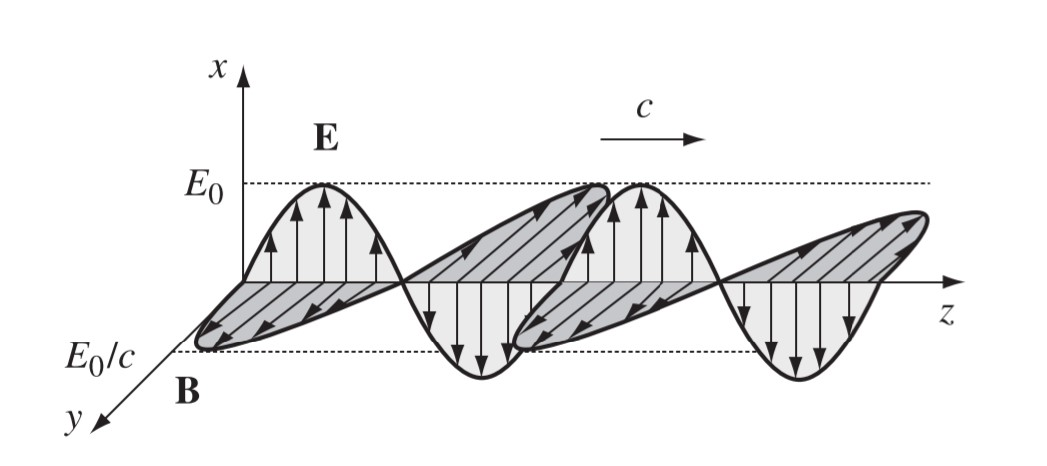
\includegraphics[width=0.7\textwidth]{Images/emwave.jpg}
    \end{figure}
\end{frame}

\begin{frame}{Poynting Vector}
    We know the energy density is,
    \begin{equation}
        u = \frac{1}{2} \left( \epsilon_0 E^2 + \frac{1}{\mu_0} B^2 \right) = \epsilon_0 E^2
    \end{equation}

    We then define the energy flux (energy per unit area, per unit time) as Poynting vector.

    \begin{block}{Poynting Vector}
        \begin{equation}
            \va{S} = \frac{1}{\mu_0} (\va{E} \times \va{B})
        \end{equation}
    \end{block}

    For the sinusoidal waves, $\va{S} = cu \vu{z}$ where $u$ is energy density.
\end{frame}

\begin{frame}{Reflection and Refraction}
    \begin{columns}
        \begin{column}{.3\linewidth}
            \begin{figure}[htbp]
                \centering
                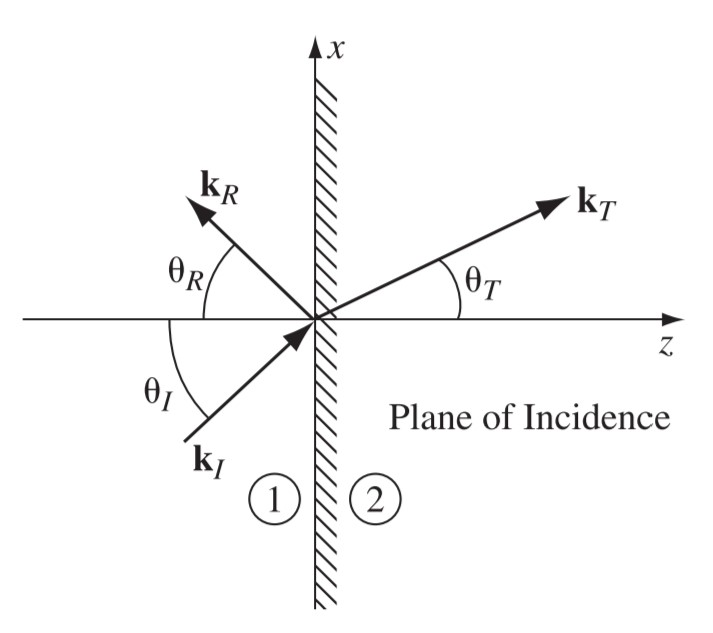
\includegraphics[width=\textwidth]{Images/re.jpg}
            \end{figure}
        \end{column}
        \begin{column}{.7\linewidth}
            \begin{block}{Law of reflection}
                \begin{equation}
                    \theta_I = \theta_R
                \end{equation}
            \end{block}

            \begin{block}{Law of refraction (Snell's law)}
                \begin{equation}
                    \frac{\sin \theta_T}{\sin \theta_I} = \frac{n_1}{n_2}
                \end{equation}
            \end{block}
            \begin{itemize}
                \item $n_i = v_i / c$ is called refractive index.
                \item When $\theta_I > \theta_{cr}$, where $\sin \theta_{cr} = n_2 / n_1$, there is a total internal reflection.
            \end{itemize}
        \end{column}
    \end{columns}
\end{frame}

\begin{frame}{Huygens' Principle}
    \begin{block}{Huygens' principle}
        Every point of the wavefront may be considered as a source of secondary wavelets that propagate out in all directions with speed equal to speed of propagation of the wave.
    \end{block}

    \begin{figure}[htbp]
        \centering
        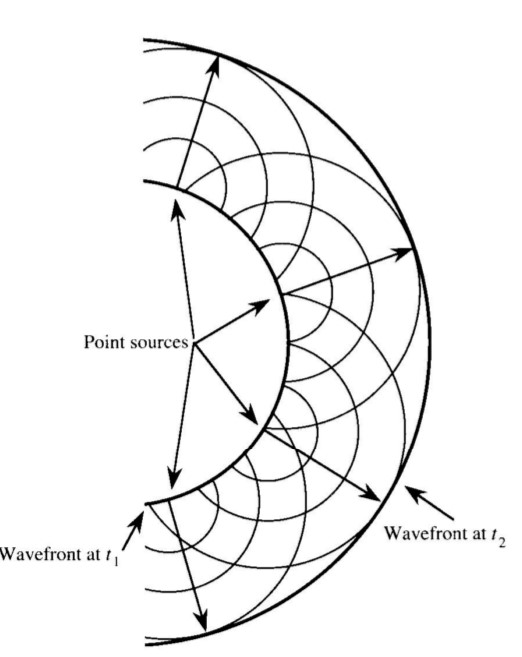
\includegraphics[height=0.5\textheight]{Images/huygens.jpg}
    \end{figure}
\end{frame}

%----------------------------------------------------------------------------------------
%	 Section 2
%----------------------------------------------------------------------------------------

\section{Exercise}


\begin{frame}{Exercise 1}
    Calculate the intensity of the standing wave represented by,
    \begin{equation}
        \va{E}(z, t) = -2E_0 \sin(kz)\sin(\omega t) \vu{x}
    \end{equation}
    \begin{equation}
        \va{B}(z, t) = -2B_0 \cos(kz)\cos(\omega t) \vu{y}
    \end{equation}

\end{frame}


\begin{frame}{Exercise 2}
    Check that $\tilde{\vb{E}}(\va{r}) = \tilde{\vb{E}}_0 e^{i(\va{k} \vdot \va{r} - \omega t)}$ and $\tilde{\vb{B}}(\va{r}) = \tilde{\vb{B}}_0 e^{i(\va{k} \vdot \va{r} - \omega t)}$ where $\abs{\tilde{B}_0} = \abs{\tilde{E}_0} / c$ satisfy the e-m wave equations.
\end{frame}

\begin{frame}{Exercise 3}
    Prove the law of reflection and refraction by Huygens' principle.
\end{frame}


%	 CLOSING/SUPPLEMENTARY SLIDES
%----------------------------------------------------------------------------------------
\section{Appendix}


\begin{frame}
    \begin{center}
        \LARGE\bf Thanks for listening!
    \end{center}
\end{frame}


%----------------------------------------------------------------------------------------

\begin{frame}{\bf References}
    \nocite{*} % Display all references regardless of if they were cited
    \bibliography{example.bib}
    \bibliographystyle{plain}
\end{frame}

\end{document}

